\section{Einfaches Beispiel}

\begin{frame}
    \frametitle{Einfaches Beispiel}

    Matrix $A$ und Vektor $\vec{b}$:
    \begin{columns}[c]
        \begin{column}{0.5\hsize}\centering
            $$A = \begin{pmatrix} 1 & -\frac{1}{3}\\ -\frac{1}{3} & 1\\ \end{pmatrix}$$
        \end{column}

        \begin{column}{0.5\hsize}
            $$\vec{b} = \begin{pmatrix} 0 \\ 1\\ \end{pmatrix}$$
        \end{column}
    \end{columns}
 
    \hfil

    \hfil

\onslide<2>{
    Klassische Lösung
    \begin{columns}[c]
        \begin{column}{0.5\hsize}
            \centering
            $$\vec{x} = \begin{pmatrix} \frac{3}{8}\\ \frac{9}{8}\\ \end{pmatrix}$$
        \end{column}

        \begin{column}{0.5\hsize}
            \centering
            Verhältnis der Lösung:
            $$\frac{ |x_0|^2}{ |x_1|^2}= \frac{\frac{9}{64}}{\frac{81}{64}} = \frac{1}{9}$$
        \end{column}
    \end{columns}
 }


\end{frame}

\begin{frame}
    \frametitle{Einfach Beispiel}


    Eigenvektoren von $A$ sind:    
    \begin{columns}[c]
        \begin{column}{0.5\hsize}\centering
            $$ \vec{u_0} = \begin{pmatrix} \frac{-1}{\sqrt{2}}\\ \frac{-1}{\sqrt{2}}\\ \end{pmatrix}$$
        \end{column}
        \begin{column}{0.5\hsize}
            $$\vec{u_1} = \begin{pmatrix} \frac{-1}{\sqrt{2}}\\ \frac{1}{\sqrt{2}}\\ \end{pmatrix}$$
        \end{column}
    \end{columns}

    \hfil

    \hfil

\onslide<2>{
    Enkodiert
    \begin{columns}[c]
            \begin{column}{0.5\hsize}\centering
                $$ \ket{u_0} = \frac{-1}{\sqrt{2}}\ket{0} + \frac{-1}{\sqrt{2}}\ket{1}$$
            \end{column}
            \begin{column}{0.5\hsize}
                $$\ket{u_1}= \frac{-1}{\sqrt{2}}\ket{0} + \frac{1}{\sqrt{2}}\ket{1}$$
            \end{column}
        \end{columns}

}
\end{frame}

\begin{frame}
    \frametitle{Einfach Beispiel}

    Eigenvektoren von $A$ sind:    
    \begin{columns}[c]
        \begin{column}{0.5\hsize}\centering
            $$\lambda_0 = \frac{2}{3}$$
        \end{column}

        \begin{column}{0.5\hsize}
            $$\lambda_1 = \frac{4}{3}$$
        \end{column}
    \end{columns}

    \hfil

    \hfil

\onslide<2>{
    Einkodiert:
    \begin{columns}[c]
        \begin{column}{0.5\hsize}\centering
            $$\ket{\widetilde{\lambda_0}} = \ket{01}$$
        \end{column}

        \begin{column}{0.5\hsize}
            $$\ket{\widetilde{\lambda_1}} = \ket{10}$$
        \end{column}
    \end{columns}
}
\end{frame}




\begin{frame}
    \frametitle{Ablauf}

    \begin{center}
    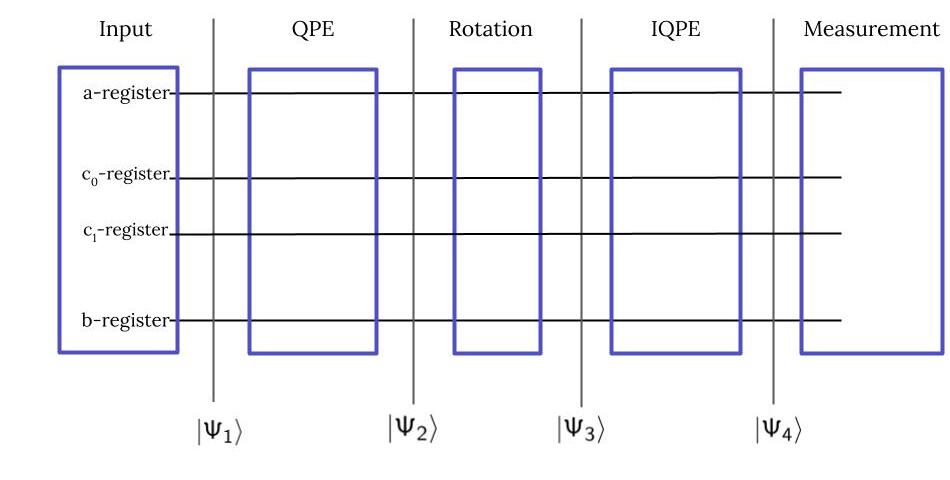
\includegraphics[width=10.5cm]{img/example_circuit/example_circuit.jpg}
    \end{center}

    \begin{enumerate}
        \item Anzahl Qubit for a-register: 1
        \item Anzahl Qubits für das c-Register: N = 2
        \item Anzahl Qubits für $\vec{b}$: $n_b = log_2(N) = log_2 (2) = 1$ 
    \end{enumerate}
\end{frame}

\begin{frame}
    \frametitle{State Preparation}

    \begin{itemize}
        \item $\vec{b}$ wird als Quantenzustand $\ket{b}$ kodiert
        \item in unserem Fall ist es sehr einfach
    \end{itemize}

    $$\vec{b} = \begin{pmatrix} 0\\ 1\\ \end{pmatrix} \Leftrightarrow \ket{b} = 0 \ket{0} + 1 \ket{1} = \ket{1}$$
\end{frame}


\begin{frame}
    \frametitle{State Preparation}

    \begin{center}
    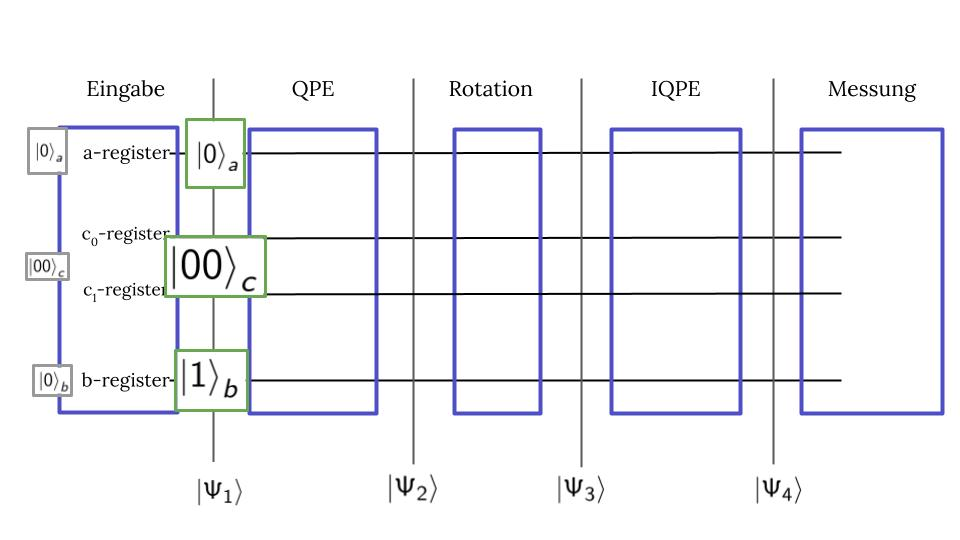
\includegraphics[width=10.5cm]{img/example_circuit/example_circuit_1.jpg}
    \end{center}

    Wir starten im 1 Zustand
    $$\ket{\Psi_1} = \ket{1}_b\ \ket{00}_c\ \ket{0}_a = \ket{1000}$$

\end{frame}


\begin{frame}
    \frametitle{Quantum Phase Estimation}
    \begin{center}
    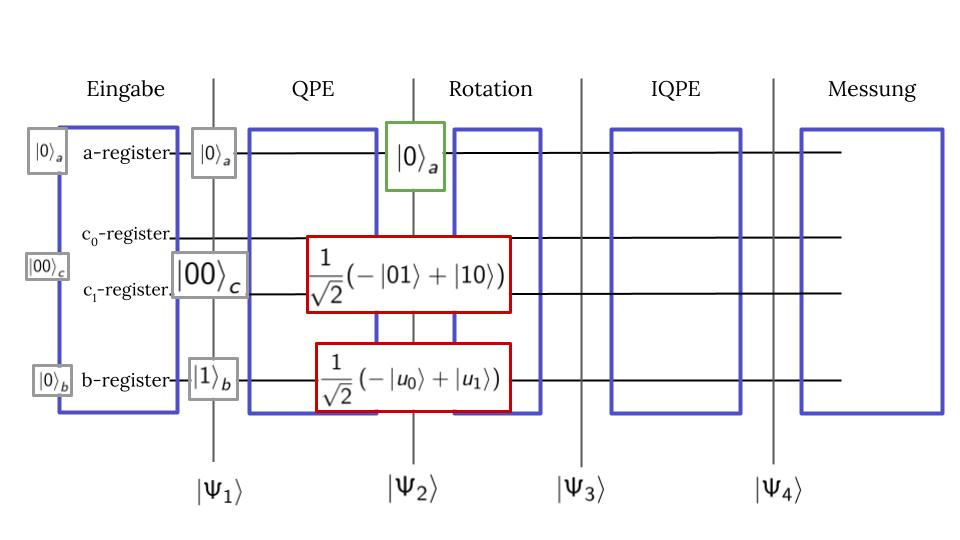
\includegraphics[width=10.5cm]{img/example_circuit/example_circuit_2.jpg}
    \end{center}

    Wir erhalten:
    $$\ket{\Psi_2} = \ket{b}_b \ket{\widetilde{\lambda}}_c\ket{0}_a$$
    $$\ket{\Psi_2} =\left(-\frac{1}{\sqrt{2}} \ket{u_0} \ket{01} +\frac{1}{\sqrt{2}}  
    \ket{u_1} \ket{10} \right)  \ket{0}_a$$

\end{frame}

\begin{frame}
    \frametitle{Ancilla Roation - Eigenwerte invertieren}
    Wir invertieren das Ancilla Qubit:
    $$ \ket{\Psi_3} = \sum_{j=0}^{2^{1}-1} b_j \ket{u_j} \ket{\widetilde{\lambda}_j} \left(\sqrt{1-\frac{C^2}{\widetilde{\lambda}_j^2}}\ket{0} + \frac{C}{\widetilde{\lambda}_j} \ket{1}\right)$$
    %$$=-\frac{1}{\sqrt{2}} \ket{u_0} \ket{01}\left(\sqrt{1-\frac{1}{1^2}}\ket{0} + \frac{1}{1} \ket{1}\right) +\frac{1}{\sqrt{2}}  \ket{u_1} \ket{10} \left(\sqrt{1-\frac{1}{2^2}}\ket{0} + \frac{1}{2} \ket{1}\right)$$
    %$$=\left(-\frac{1}{\sqrt{2}} \ket{u_0} \ket{01}\left(\ket{0} +\ket{1}\right)+\frac{1}{\sqrt{2}} \ket{u_1} \ket{10}\right)\left(\sqrt{1-\frac{1}{4}}\ \ket{0} + \frac{1}{2} \ket{1}\right)$$


    \hfil

    Wir gehen davon aus, dass wir $\ket{1}$ messen.
    $$  \ket{\Psi_3} =\sqrt{\frac{8}{5}}\left(-\frac{1}{\sqrt{2}} \ket{u_0}_b\ket{01}_c +\frac{1}{2\sqrt{2}} \ket{u_1}_b\ket{10}_c\right)\ket{1}_a $$
\end{frame}

\begin{frame}
    \frametitle{Ancilla Roation - Eigenwerte invertieren}
    \begin{center}

    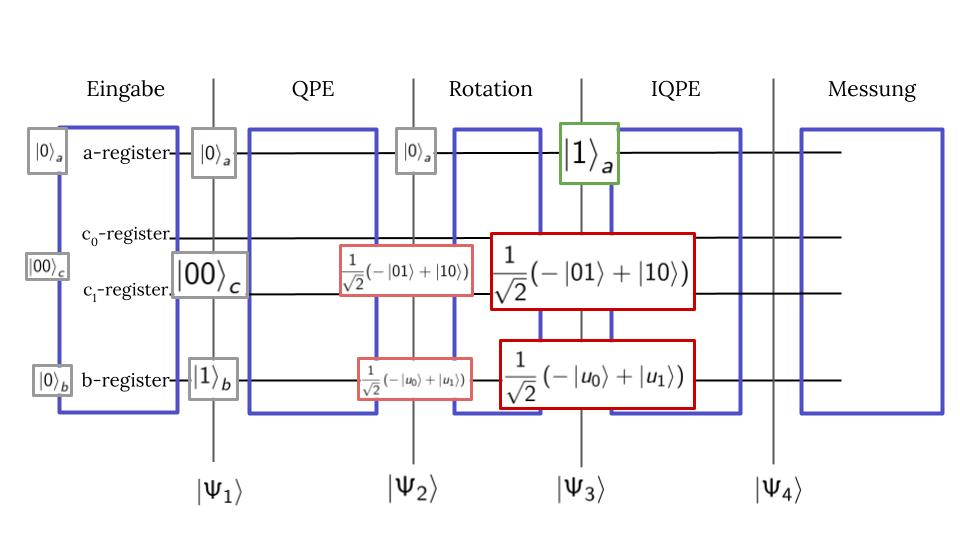
\includegraphics[width=10.5cm]{img/example_circuit/example_circuit_3.jpg}
    \end{center}
    $$ \ket{\Psi_3} =\sqrt{\frac{8}{5}}\left(-\frac{1}{\sqrt{2}} \ket{u_0}\ket{01}\ket{1} +\frac{1}{2\sqrt{2}} \ket{u_1} \ket{10}\right)\ket{1}_a$$
\end{frame}

\begin{frame}
    \frametitle{Inverse Quantum Phase Estimation}
    \begin{center}
    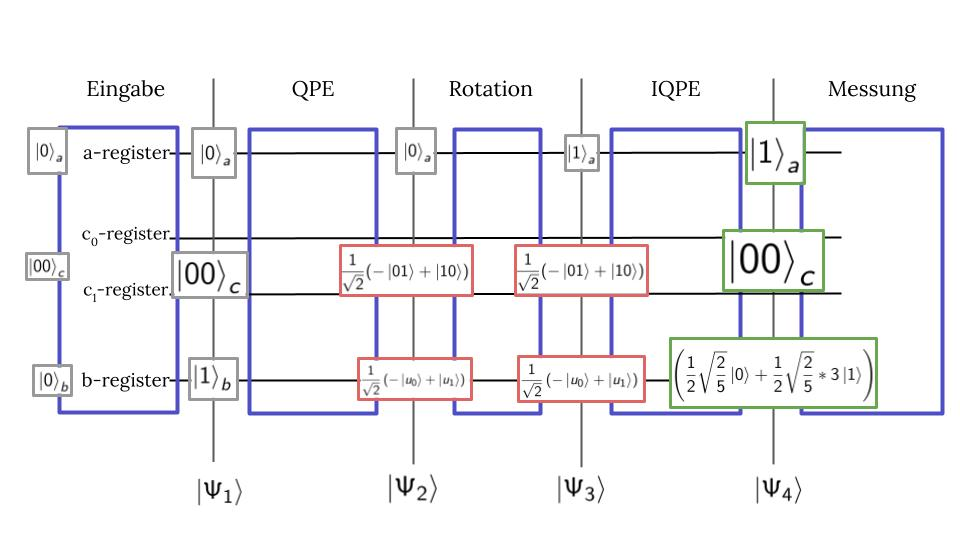
\includegraphics[width=10.5cm]{img/example_circuit/example_circuit_4.jpg}
    \end{center}

Wir erhalten:
$$\ket{\Psi_4}= \ket{x}_b \ket{00}_c \ket{1}_a $$
$$ \ket{\Psi_4}=\frac{1}{2}\sqrt{\frac{2}{5}}  \left(\ket{0} +3 \ket{1} \right) \ket{00}_b \ket{1}_a$$
\end{frame}


\begin{frame}
    \frametitle{Measurment}

Um die Wahrscheinlichkeit von $ \ket{u_0}$ und $\ket{u_1}$ zu erhalten, müssen wir ihre Koeffizienten quadrieren

$$ c_0=\left|\frac{1}{2}\sqrt{\frac{2}{5}}*1\right|^2 = \frac{1}{20} $$

$$ c_1=\left|\frac{1}{2}\sqrt{\frac{2}{5}}*3\right|^2 = \frac{9}{20} $$

Das Verhältnis im b-Register ist wie erwartet $1:9$.

\end{frame}






